Los requisitos se dividieron en grupos a modo de facilitar el trabajo sobre cada uno de ellos, de forma tal que la funcionalidad base pudiera dar cuenta de un conjunto de ellos en lugar de tan solo uno. Por ejemplo, si el sistema requiere de la inscripción de un usuario, era necesario que el usuario pudiera crear su cuenta, pudiera inscribirse y pudiera salir de su cuenta. \\
De esta forma, los requisitos se dividieron en: Requisitos generales (1-2, 4) Sistema de reservas y prestamos (5, 7-8, 12, 14-15), landing page para personas naturales (16-18), perfil de usuario (23, 25-26, 28), ficha de artículo (37-40), landing page para administradores (51, 54-56). \\
Del primer grupo de requisitos, podemos ver como estos se cumplen en las siguientes imágenes:

\begin{figure}[H]
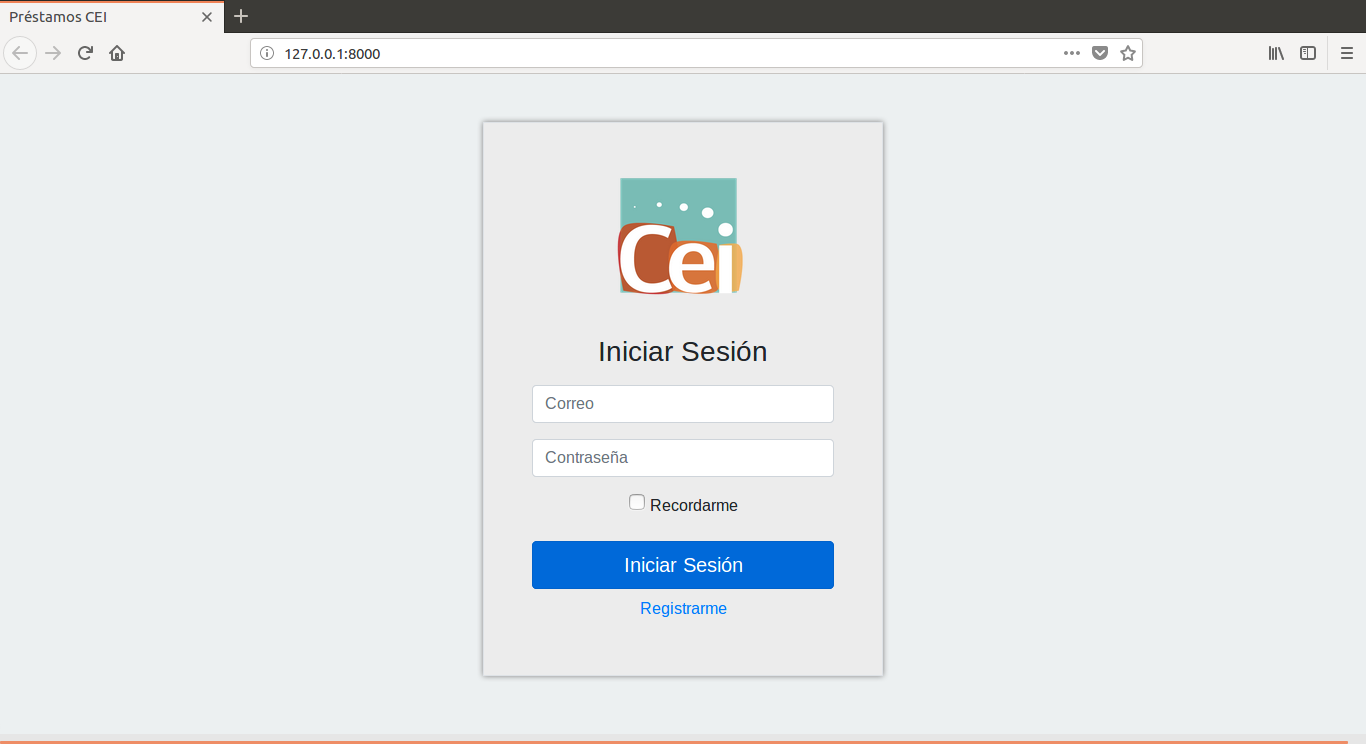
\includegraphics[width=0.5\textheight]{images/login.png}
\caption{Página inicial de recepción a usuarios sin cuenta. Pide iniciar sesión (req 2) o crear cuenta (req 1) para poder acceder a los servicios del sistema.} \label{Login}
\end{figure}

\begin{figure}[H]
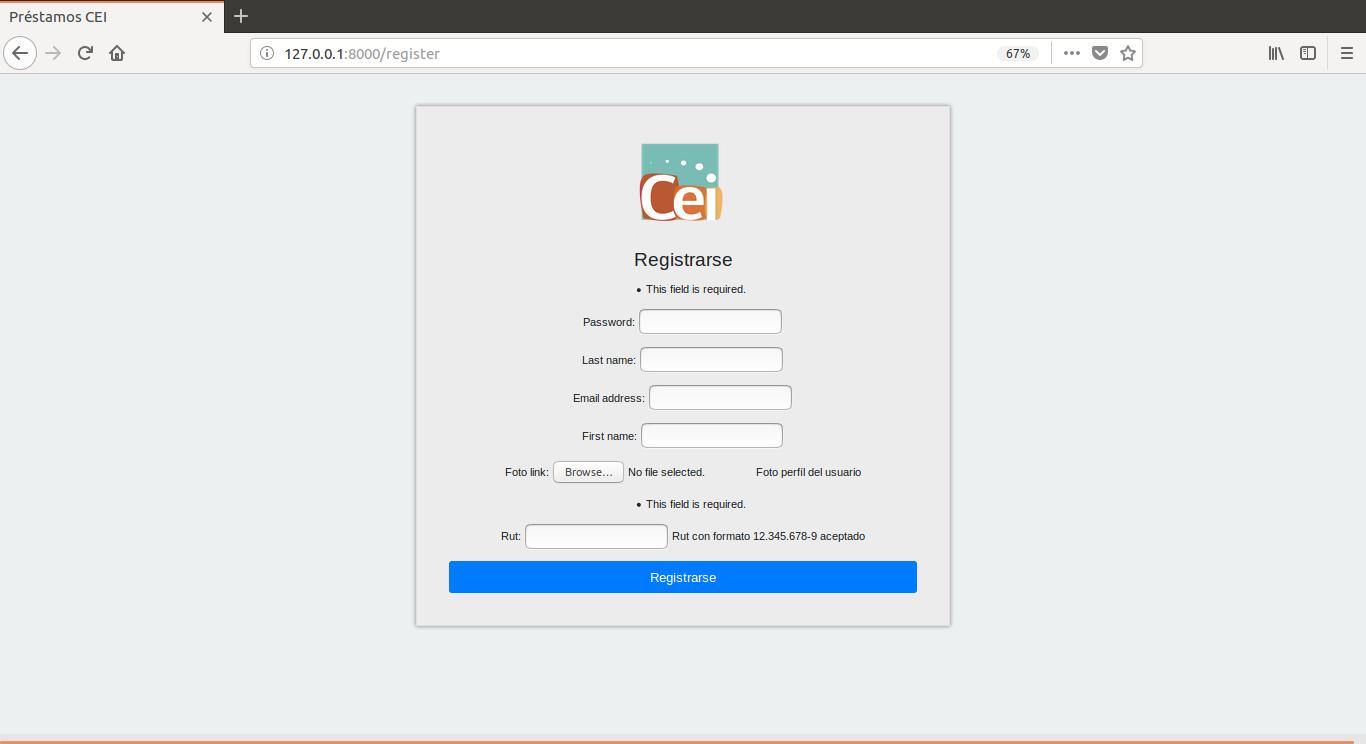
\includegraphics[width=0.5\textheight]{images/registro.png}
\caption{Página de creación de usuario (req 1). Todo usuario creado de esta forma es una persona natural, y solo los administradores pueden cambiar una cuenta a cuenta de administración (req 4).} 
\label{Registro}
\end{figure}

Del sistema de reservas y prestamos, podemos apreciar como se resuelven los requisitos establecidos en la siguiente imagen de la interfaz que se implementa: \\

\begin{figure}[H]
%\includegraphics[width=0.5\textheight]{//.png}
\caption{Se aprecia como funciona el sistema de solicitud de prestamos. Se puede observar que solo se pueden solicitar durante los días habiles (req 14), pero otros detalles como las restricciones de tiempo (req 12) e identificadores únicos (req 15) no se puede apreciar por su propia naturaleza interna.} 
\label{Solicitar}
\end{figure}

De los requisitos asociados al landing page para personas naturales, podemos ver como estos se cumplen en las siguientes imágenes:


\begin{figure}[H]
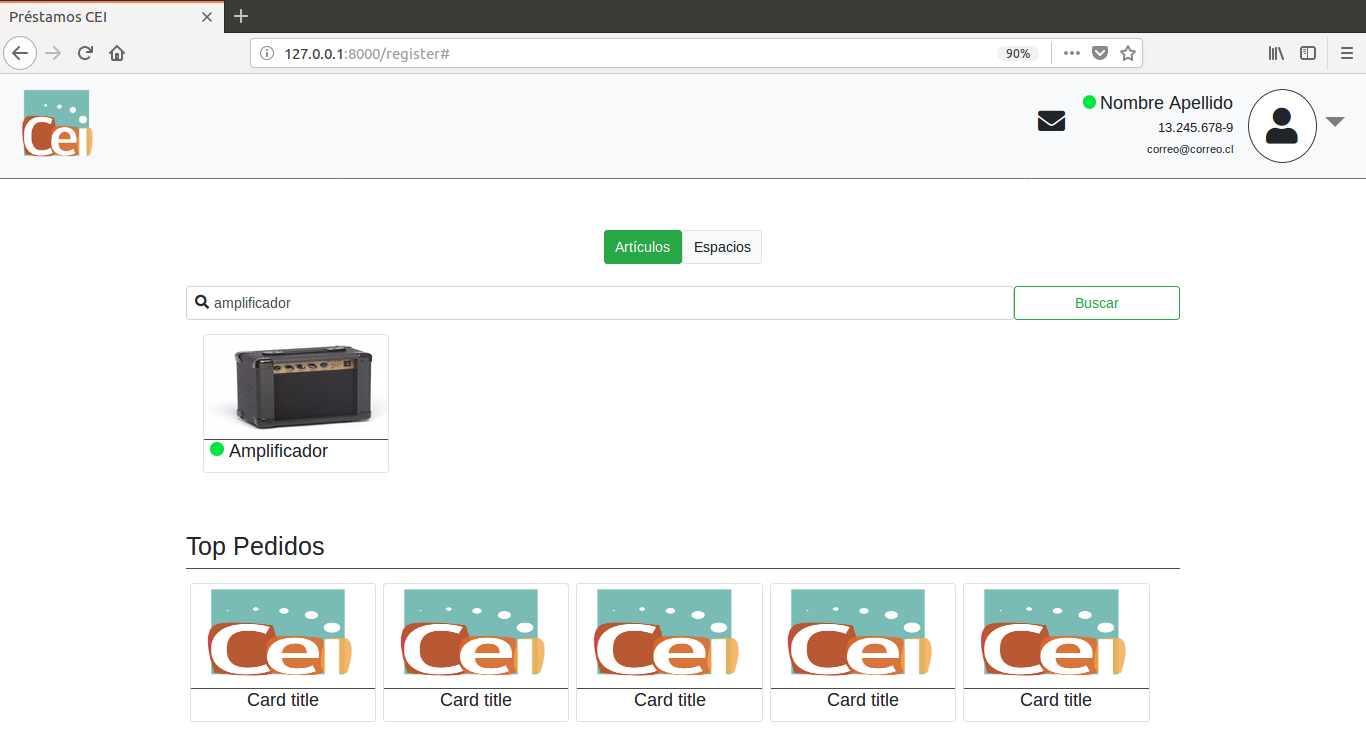
\includegraphics[width=0.5\textheight]{landing-page.png}
\caption{Página de inicio para persona natural recién conectada. Se puede apreciar como el usuario puede buscar artículos (req 16) y la barra de navegación a su perfil e historial de pedidos (req 23). Adicionalmente, se puede apreciar como la busqueda se puede restringuir según los criterios seleccionados por el usuario (req 17).} 
\label{LPUsers}
\end{figure}

\begin{figure}[H]
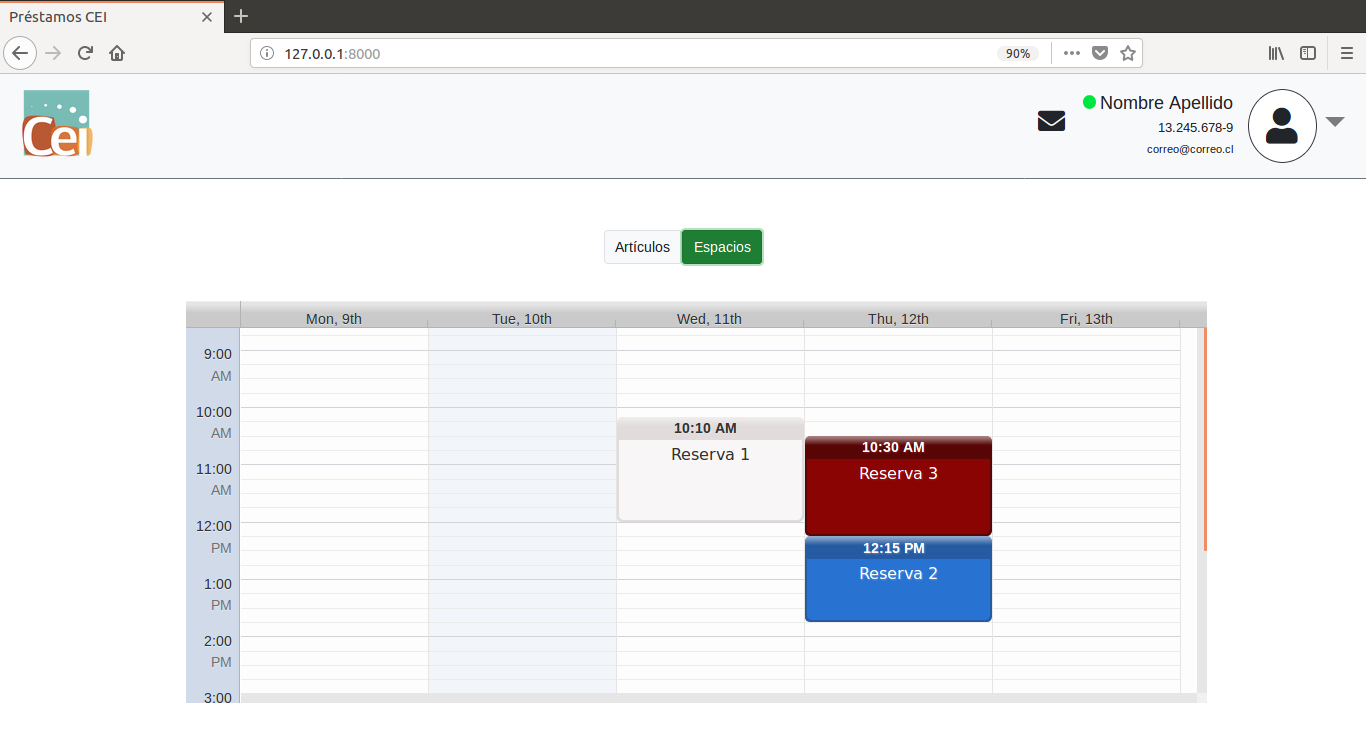
\includegraphics[width=0.5\textheight]{landing-page-espacios.png}
\caption{Página de inicio para persona natural, en pestaña de busqueda de espacios. Se aprecia la "grilla" con los horarios de espacios reservados (req 18).} 
\label{LPUsersEspacios}
\end{figure}

Respecto del perfil de usuario, los requisitos que aquí se cumplen son los siguientes:


\begin{figure}[H]
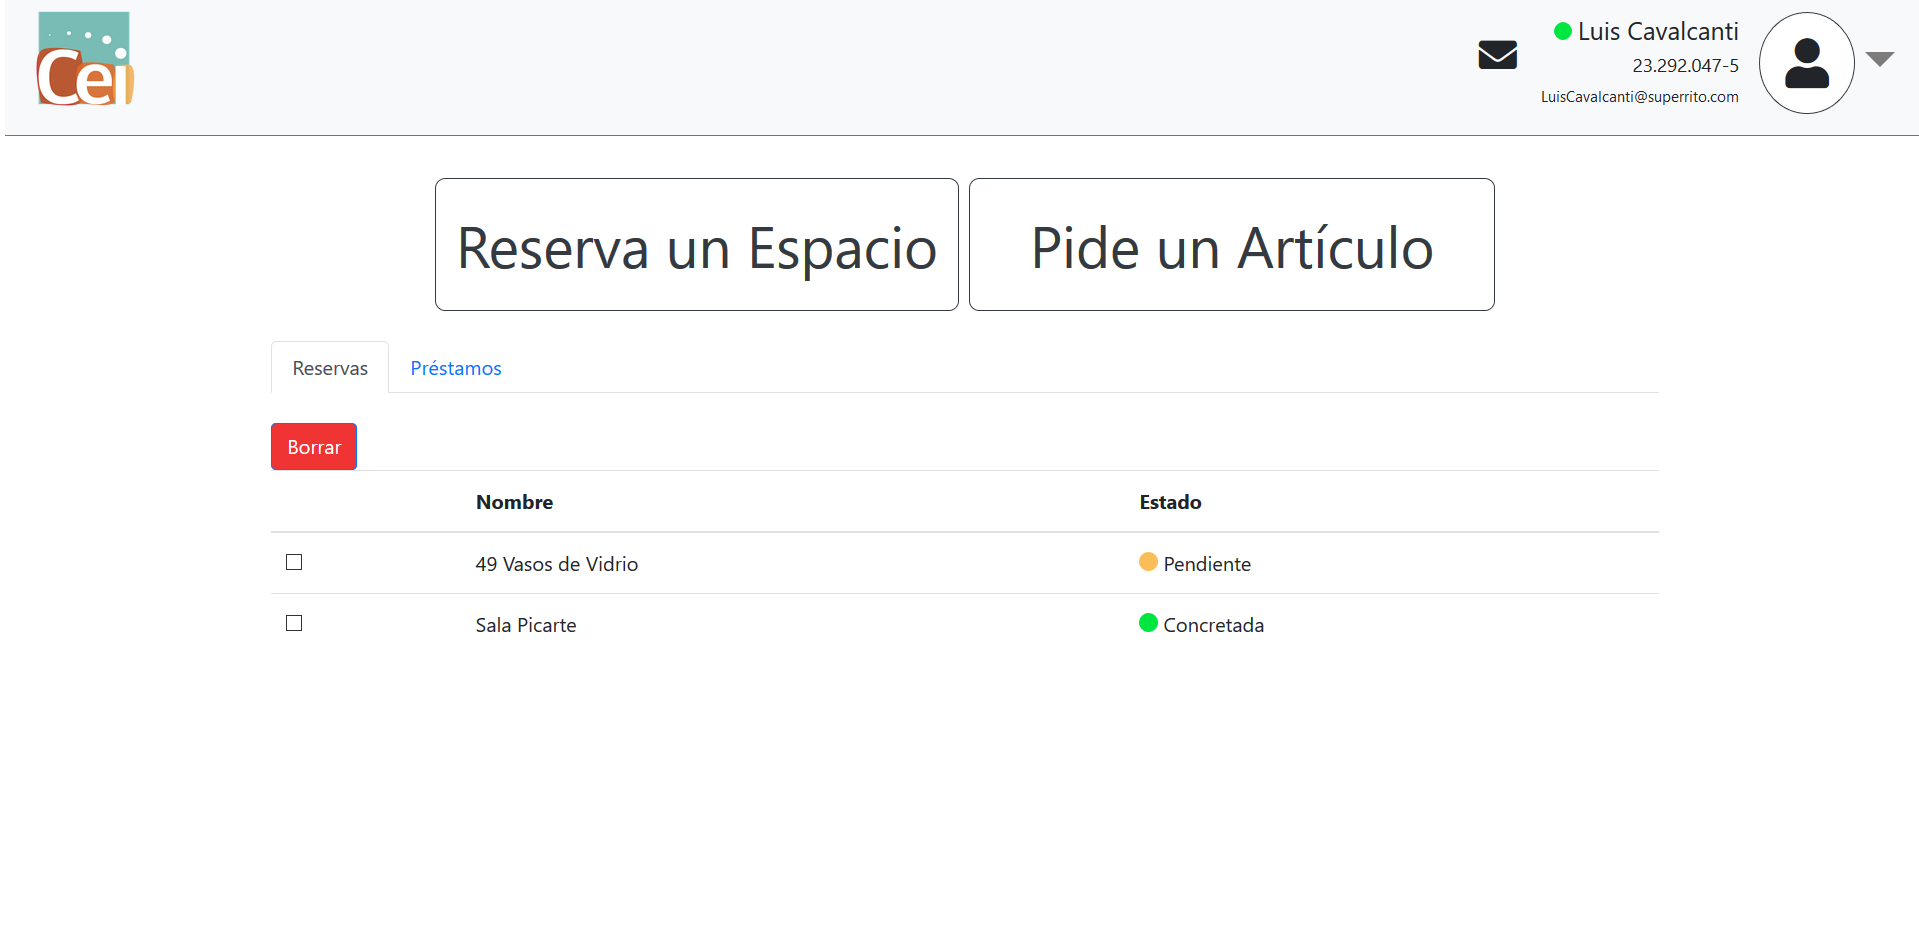
\includegraphics[width=0.5\textheight]{perfil-user.png}
\caption{Página de perfil del usuario (visto por su dueño). En esta imagen se puede apreciar los elementos propios del usuario (req 23), así como la disponibilidad de su cuenta para crear y concretar prestamos y reservas (req 25). Adicionalmente, se presenta un historial con las últimas 10 reservas realizadas por el usuario (req 7 y 26) y muestra la posibilidad de eliminarlas si estas aún no se concretan (req 28).} 
\label{LPUsersEspacios}
\end{figure}

Por otra parte, de los requisitos asociados a la ficha del artículo, las siguientes imágenes muestran como se concretan y resuelven dichos requisitos:

\begin{figure}[H]
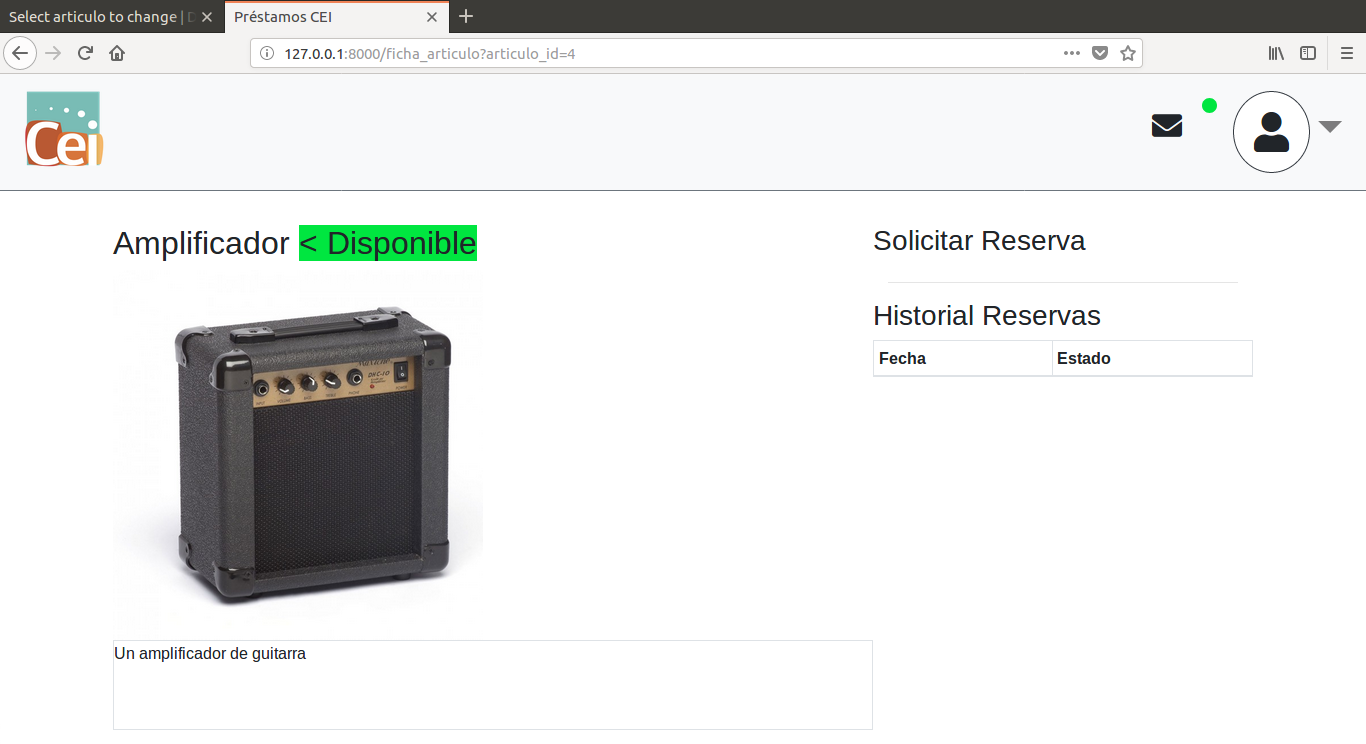
\includegraphics[width=0.5\textheight]{ficha_articulo.png}
\caption{Página correspondiente a la ficha del artículo. Se puede apreciar como el artículo dispone de toda la información solicitada (req 37), junto con un resumen de los últimos pedidos hechos por el artículo (req 38). También se observa como el usuario, persona natural, puede hacer una solicitud de prestamo por este artículo (req 5 y 40).]
[Ficha del artículo (vista admin)/ comentario: Página correspondiente a la ficha del artículo, visto por la cuenta de un administrador. Se ven los mismos elementos que en la vista por una persona natural, pero se añade la posibilidad de gestionar la información del artículo por el administrador (req 39).} 
\label{FichaArt}
\end{figure}

Finalmente, los requisitos asociados directamente con la landing page de los administradores se pueden ver en las siguientes imágenes del sistema, vistos por una cuenta de administrador:

\begin{figure}[H]
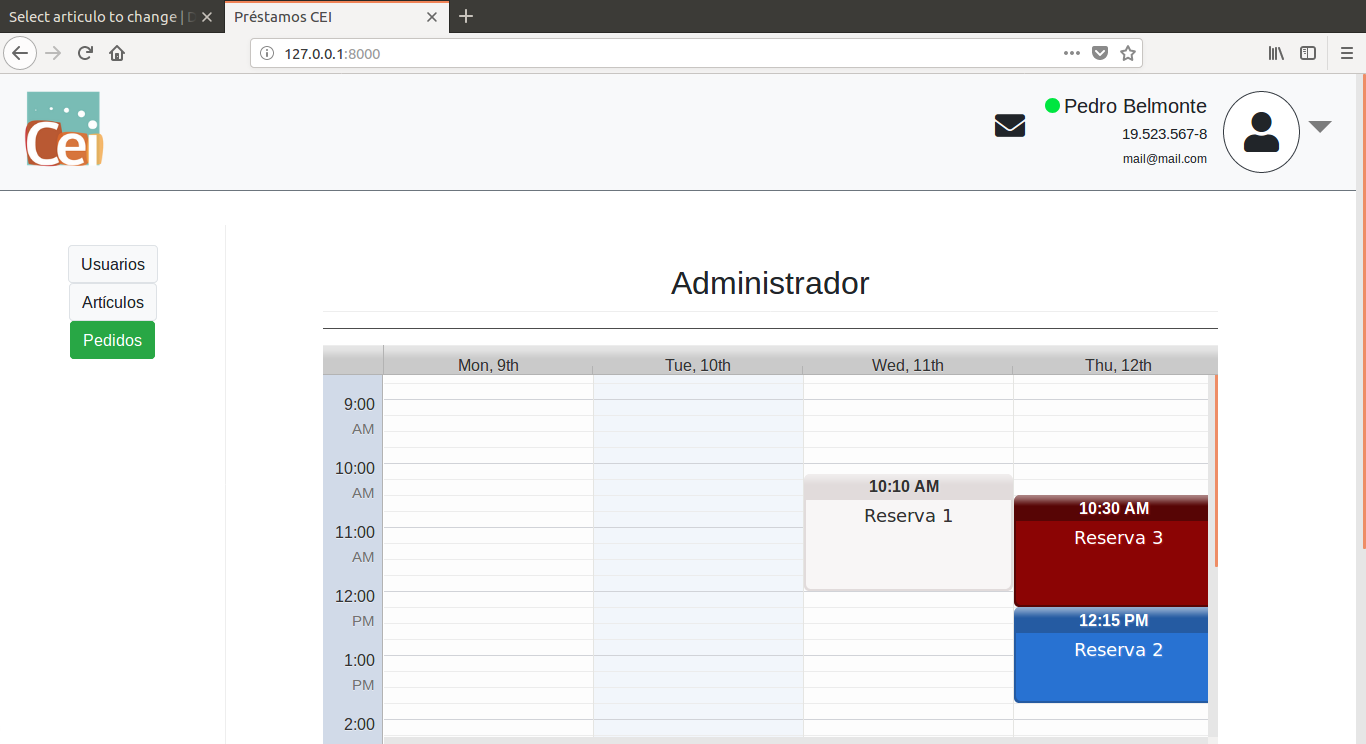
\includegraphics[width=0.35\textheight]{landing-admin1.png}
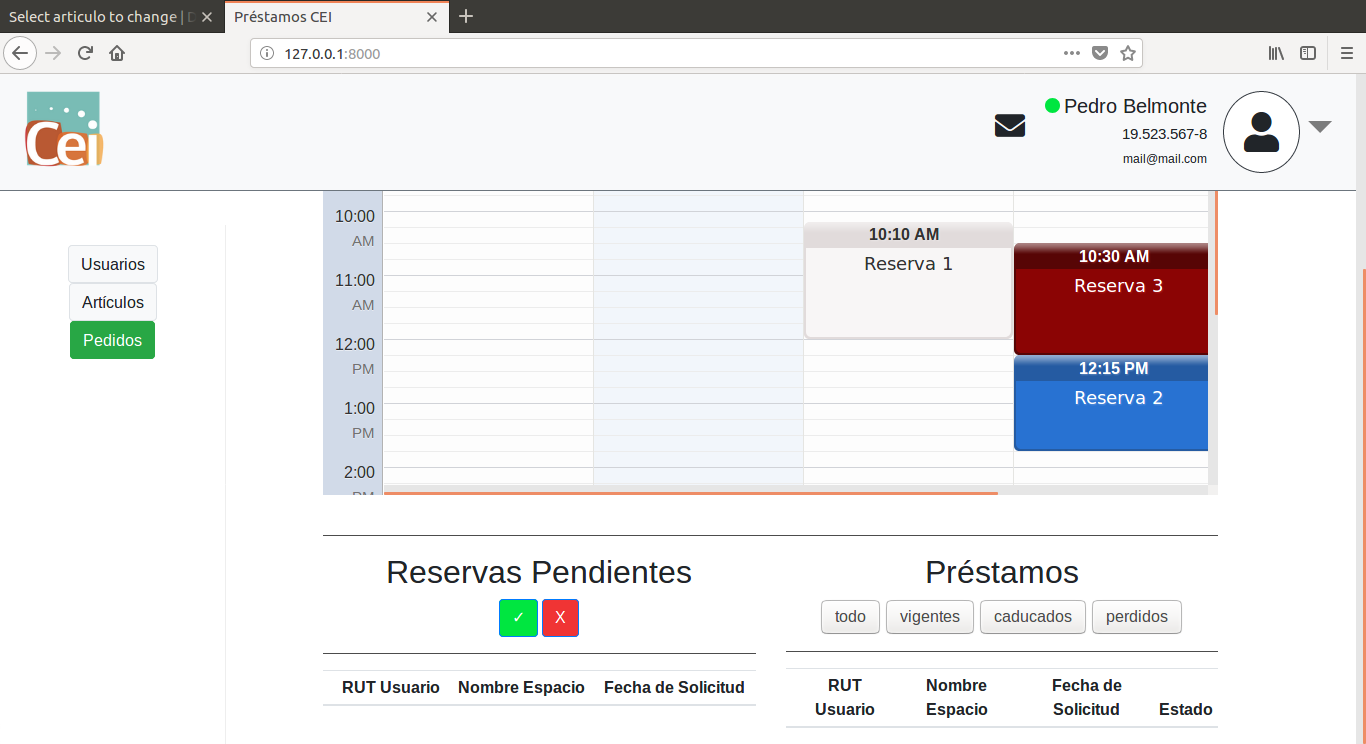
\includegraphics[width=0.35\textheight]{landing-admin2.png}
\caption{Página inicial de recepción para un administrador. Se aprecia el sistema de "grilla" para los horarios de reserva para los espacios administrados por el CEI (req 51). Se aprecian las reservas pendientes ordenadas por fecha (req 54), la posibilidad del administrador de marcas dichas reservas (req 55).} 
\label{LPAdmin}
\end{figure}


\begin{figure}[H]
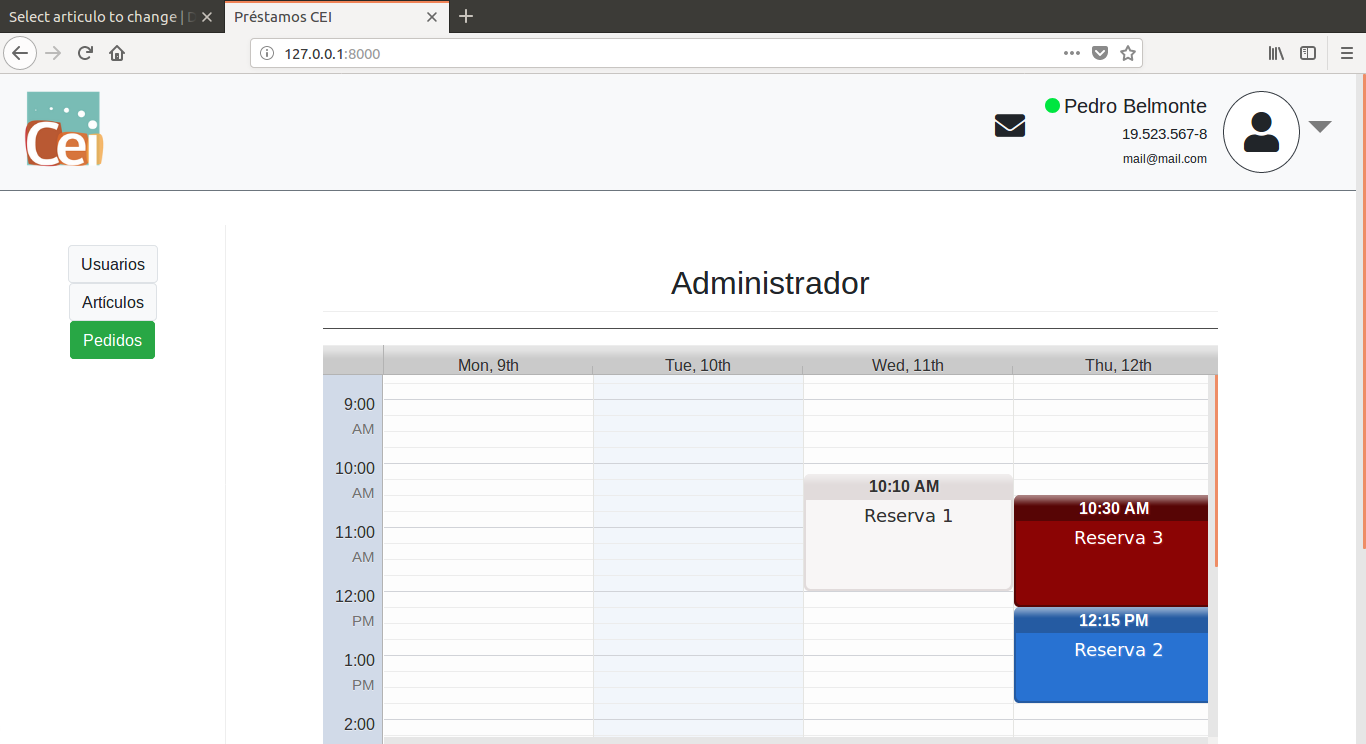
\includegraphics[width=0.35\textheight]{landing-admin1.png}
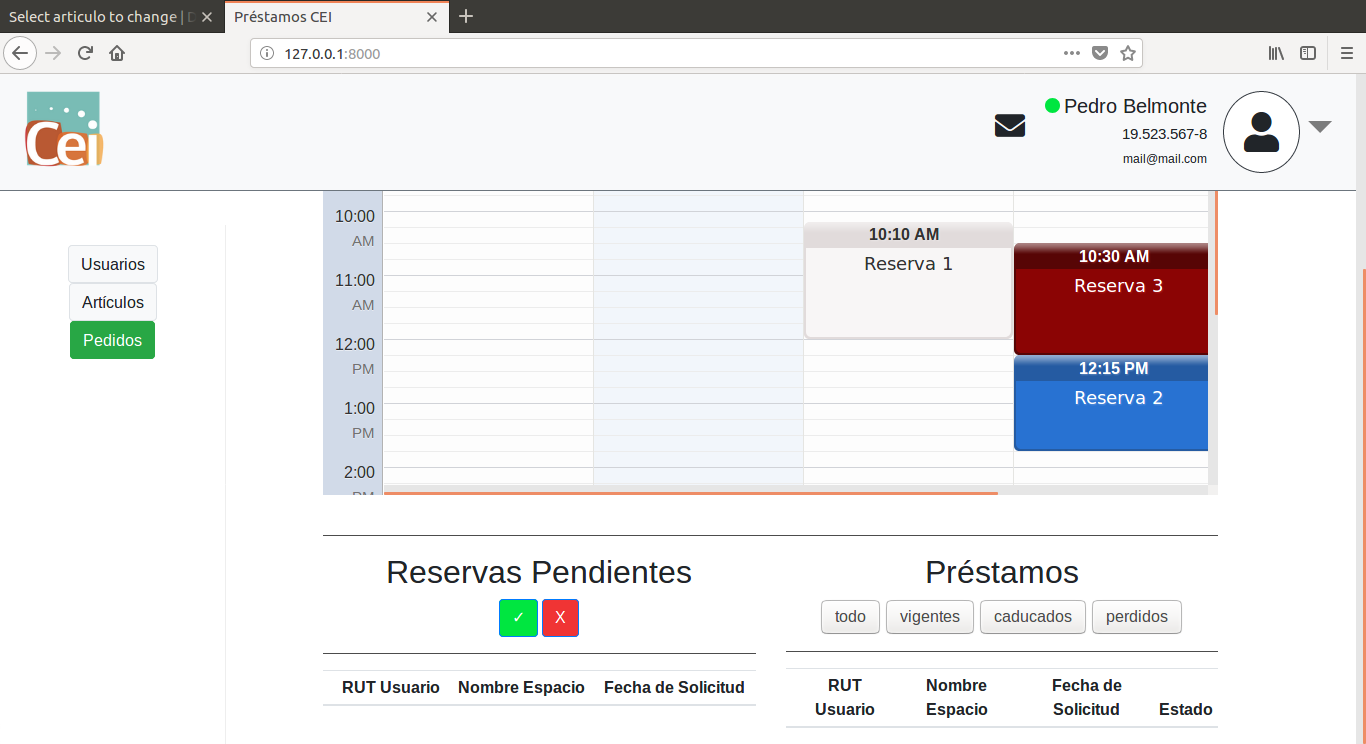
\includegraphics[width=0.35\textheight]{landing-admin2.png}
\caption{LP de admin con prestamos pendientes/comentarios: Página inicial de recepción para un administrador, con listado de préstamos pendientes. Se aprecia el orden de los préstamos pendientes y la posibilidad de filtrar por estado (req 8 y 56).}
\label{LPAdmin2}
\end{figure}

Cabe hacer notar que la funcionalidad desarrollada para una parte, se aprovecha también para otra parte del sistema, por lo que ciertos requisitos se cumplen más de una vez.